\subsection{Serialize RAW Data to Local Disk}

The first step of experiments are serialize various complex objects and the write into a file in disk. In this experiment, the raw tweet data set read line-by-line and convert to a objects. The serialization tasks for each of the thirteen implementation method run. In the serialization process each object serialized or copy the final serialization result into $256KB$ pages and the objects indexed in separate file.

%\begin{figure}[t]
%	\centering
%	\resizebox{\columnwidth}{1.5in}{
%		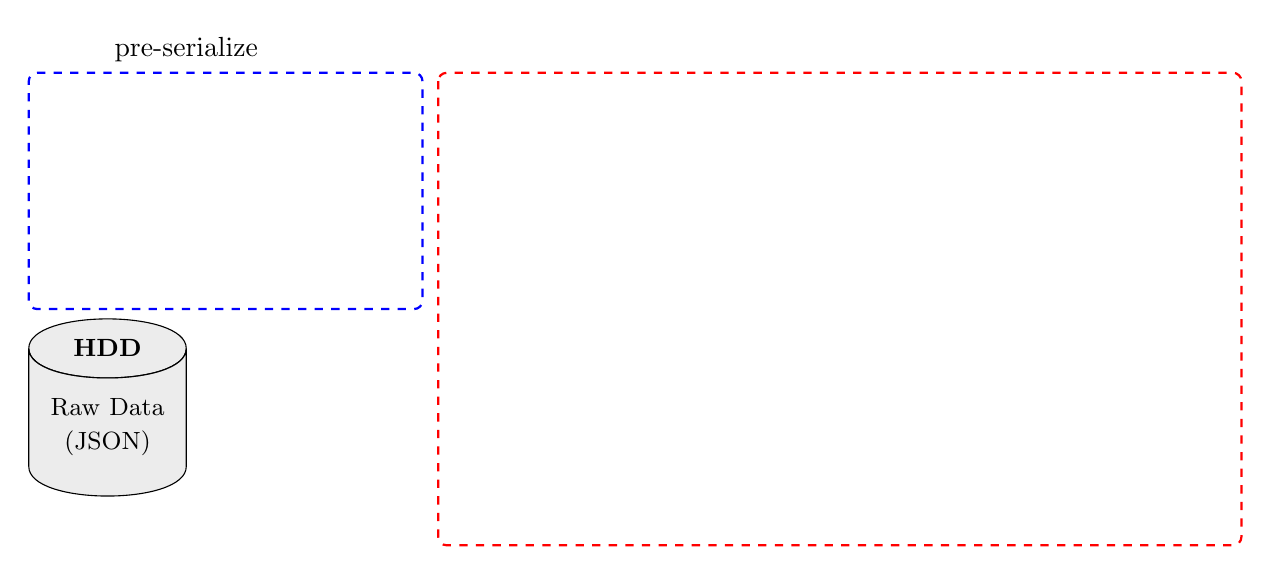
\begin{tikzpicture}
\draw (2,3.3) node{pre-serialize};
\draw[blue,thick,dashed,rounded corners=3pt](0,0) rectangle ++(5,3);
\draw[red,thick,dashed,rounded corners=3pt](5.2,3) rectangle ++(10.2,-6);

%\draw (0,0) -- (10,0) -- (10,4) -- (0,4) -- (0,0);

  \draw[fill=lightgray!60, fill opacity=0.5] (0,-0.5) to
 [controls=+(90:0.5) and +(90:0.5)] (2,-0.5);
 
 \draw[fill=lightgray!60, fill opacity=0.5] (0,-0.5) .. controls +(-90:0.5)
 and +(-90:0.5) .. (2,-0.5);
 
 \draw[fill=lightgray!60, fill opacity=0.5] (0,-0.5) .. controls +(-90:0.5)
 and +(-90:0.5) .. (2,-0.5)
 -- (2,-2) .. controls +(-90:0.5) and +(-90:0.5) .. (0,-2) -- (0,-0.5);
 
 \draw (1,-0.5) node[align=center,text width=1.5cm] {\centering\small\textbf{HDD}};
 \draw (1,-1.5) node[align=center,text width=1.5cm] {\centering\small{Raw Data (JSON)}};
 
 
 
\end{tikzpicture}
%	}
%	\caption{serialize process}
%	\label{fig:serialize_process}
%\end{figure} 

\begin{figure}
	\centering
	\includegraphics[width=\columnwidth,height=2.3in,keepaspectratio]{img/serialize_process.pdf}
	\caption{serialize process}
	\label{fig:serialize_process}
\end{figure}

\subsubsection{Results}

In Figure \ref{fig:exp_serialization_bar}, we show, for each of the thirteen implementations, for both $taskset$ TRUE and FALSE the total running time required as a function of the number of Tweet objects write experiments. In the figure where the
performance differences are easier to see; we also breakdown
the total time into I/O and CPU.
\begin{figure*}
	\centering
	\includegraphics[width=\linewidth ,height=2.5in,keepaspectratio]{../../RScripts/Experiment_SerializeObjects_Bar.pdf}
	\caption{Serialize Objects for 5M Tweets}
	\label{fig:exp_serialization_bar}
\end{figure*}

\subsubsection{Discussion}
